\documentclass[8pt]{beamer}
\usetheme{default} % Very simple theme
\usecolortheme{dove} % Minimalist grayscale colors
\setbeamertemplate{navigation symbols}{} % Remove navigation bar

% Define brand-like colors
\definecolor{myblue}{RGB}{0, 102, 204}    % Blue for standard blocks
\definecolor{mygreen}{RGB}{0, 153, 0}     % Green for example blocks
\definecolor{myred}{RGB}{204, 0, 0}       % Red for alert blocks
\definecolor{myorange}{RGB}{255, 128, 0} % For \emph

% Accent color for titles, bullets, etc.
\setbeamercolor{structure}{fg=myblue}

% Block colors
\setbeamercolor{block title}{bg=myblue, fg=white}
\setbeamercolor{block body}{bg=blue!5, fg=black}

\setbeamercolor{exampleblock title}{bg=mygreen, fg=white}
\setbeamercolor{exampleblock body}{bg=green!5, fg=black}

\setbeamercolor{alertblock title}{bg=myred, fg=white}
\setbeamercolor{alertblock body}{bg=red!5, fg=black}
\setbeamercolor{alerted text}{fg=myred}

% Optional: color for \example text
\setbeamercolor{example text}{fg=mygreen}

% Custom emph (orange text instead of italic)
\let\oldemph\emph
\renewcommand{\emph}[1]{\textcolor{myorange}{#1}}


\usepackage{graphicx} % Package for images
\usepackage{amsmath} % Package for images
\graphicspath{{figs/}} % Path to your figures directory
\usepackage{array}  % For better column spacing
\usepackage{caption} % Required for \captionof

% Title Information
\title{STOCHASTIC METHODS IN WATER RESOURCES}
\vspace{25pt}
\subtitle{Unit 4: Time series analysis \\ Lecture 11: Introduction and components of time series}
\author{Luis Alejandro Morales, Ph.D.}
\institute{Universidad Nacional de Colombia \\ Department of Civil and Agriculture Engineering} %// }
%\date{\today}

\begin{document}

% Title Slide
\begin{frame}
    \titlepage
\end{frame}

%-------
% From Kotte (Stochastic WR tech)
\section{Introduction}
\begin{frame}{Introduction}
    \begin{itemize}
        \item The \alert{analysis of time series} describe the \emph{history of the movement in time} of some hydrological variables such as the flow rate in a particular section of a river.
        \item A \alert{time series} is set of observations that measure the \emph{variation in time} of certain phenomenon e.g. flow rate, water level in a lake. 
        \item A \emph{time series} pertains to the category \emph{continuous state} and \emph{discrete time} in which observations are made of continuously changing phenomena at \emph{intervals of time } (usually equal) or an \emph{average } or \emph{total} value is taken for each time interval.
        \item \emph{Air temperature} recorded each day at noon; mean monthly \emph{barometric pressure} at a station. 
        \item The information contained in a \emph{discrete time series} is affected by the \emph{sampling interval}. 
        \item The interval depends on the purposes of the study. For instance when monitoring \emph{water quality} in a stream hourly or daily samples are recommended, whereas for studying \emph{water level} in a large reservoir, monthly data may suffice. 
        \item Optimum sample intervals can be obtained based on \emph{periodicity} and other  phenomena characteristics. 
        \item A essential characteristic of \emph{time series} is \emph{time-dependency} between observations.  So, the order of the observations is important and the smaller the time interval the stronger the relationship between observations. 
    \end{itemize}
\end{frame}

\begin{frame}{Introduction}
    \begin{itemize}
    \item A \emph{stochastic process}, $X(t)$,  is a type of \alert{random functions} defined in the \emph{time} domain. The \emph{stochastic process} is thus the collection of all possible \emph{realizations} of $X(t)$. Each \emph{realization} of $X(t)$ is \emph{uncertain} and is known as \alert{time series}, $x(t)$. In other way, $X(t)$ measures the \emph{state} of the process at an particular time $t$. 
        \vspace{-2pt}
    \begin{center}
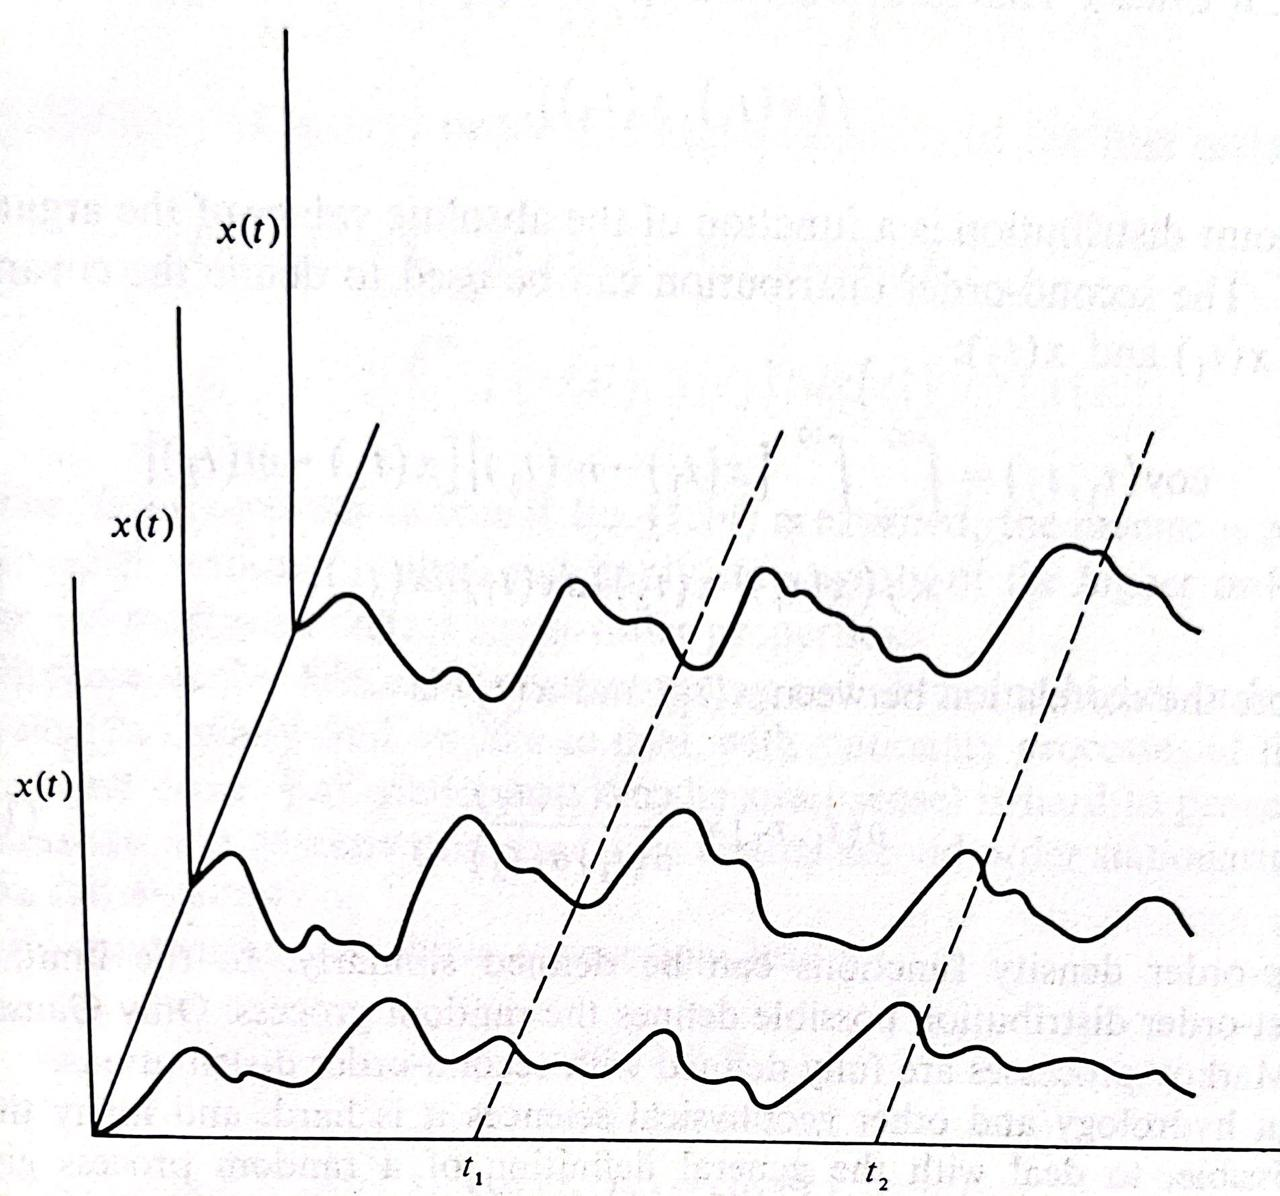
\includegraphics[width=0.6\linewidth]{fiBr12.jpeg}  % from Bras
    \end{center}

    \item The main objective in studying time series is:
        \begin{enumerate}
            \item to \emph{understand} the \emph{mechanism} that generates the data. (most important)    
            \item to \emph{simulate} likely sequences of data over period o time.
            \item to \emph{produce likely future sequences} or to \emph{forecast} events over a short period of time. Note that \emph{simulation} and \emph{forecasting} is possible by making inferences regarding the underlying laws of the \emph{stochastic process} from a sequence of observed data.
        \end{enumerate}
    \end{itemize}
\end{frame}

%-------
% From Diaz-Granados
\section{Components of time series}
\begin{frame}{Components of time series}
    \begin{block}{Generalities}
    \end{block}

    The figure below shows the components and  subdivisions of \emph{hydrological time series}.
    \begin{center}
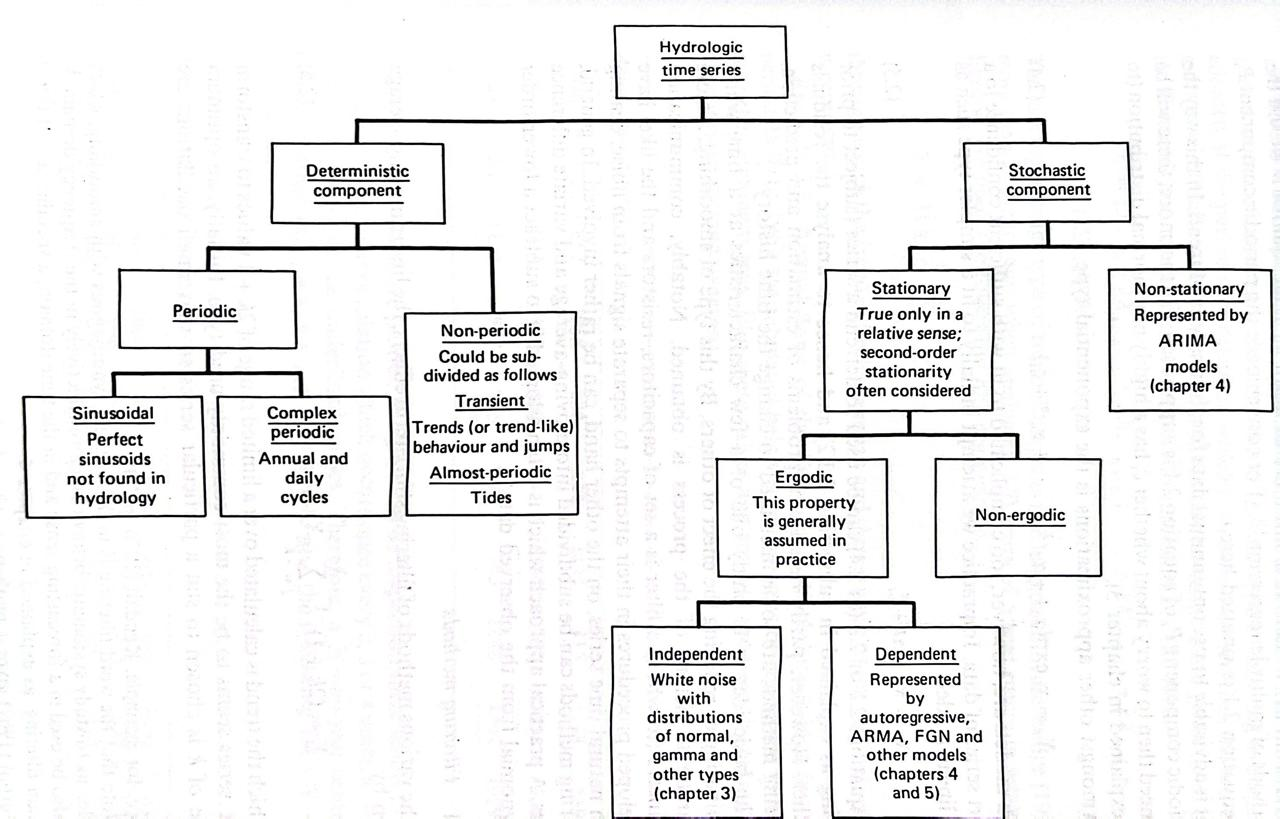
\includegraphics[width=\linewidth]{fiKo23.jpeg}  % from Kotte (stochastic..) 
    \end{center}
\end{frame}

\begin{frame}{Components of time series}
    \begin{block}{Generalities}
    \end{block}
    \emph{Hydrological time series} $x(t)$ can show different degrees of \emph{trend}, \emph{jumps} and \emph{displacements}, and also \emph{stationarity}, \emph{random fluctuations}, \emph{autocorrelation} and \emph{non Normality}. Such components can be grouped in: \alert{deterministic} and \alert{stochastic}. While the \emph{deterministic} components $d(t)$ are \emph{stationarity}, \emph{trends}, \emph{jumps} and \emph{periodicities}, the \emph{stochastic} components $\xi (t)$ is constituted by \emph{random fluctuations} that are not explained from the physical laws and thus require \emph{pdf}s and \emph{autocorrelation} function for their description. A $x(t)$ can be represented as
    \[
        x(t) = d(t) + \xi(t)
    \]
    where $d(t) = s(t) + b(t) + p(t)$ and $s(t)$, $b(t)$ and $b(t)$ represent trends, jumps and periodicities, respectively. Alternatively, $x(t)$ can be represented as
    \[
        x(t) = d(t) \xi(t)
    \]
where $d(t) = s(t) b(t) p(t)$. This equation can be transformed into a lineal equation taken logarithms in both sides. The components of the time series are described below.  
\end{frame}

\begin{frame}{Components of time series}
    \begin{block}{Trends}
    \end{block}
        \begin{itemize}
            \item \alert{Trends} are continuous and gradual \emph{increments} or \emph{declines} of the hydrological variable during certain time period.
            \item \emph{Trends} can occur during the whole time period or during part of the period. 
            \item \emph{Trends} can be attributed to \emph{natural} or \emph{anthropic} factors. For instance, \emph{land-use changes}, \emph{deforestation} and \emph{climate change} in a basin trigger long-term trends in streamflow time series. 
            \item In presence of \emph{trends}, the time series shows a \emph{positive} or \emph{negative} correlation with time. 
        \end{itemize}
        The following table show mathematical functions to represent \emph{trends}.
\begin{minipage}[]{0.48\textwidth}
    \begin{center}
  \begin{tabular}{|l|c|}
      Linear & $\bar{x}(t) = a + bt$ \\
      Polynomial & $\bar{x}(t) = a + bt + ct^2$ \\
      Power & $\bar{x}(t) = at^b$ \\
      Reciprocal & $\bar{x}(t) = \frac{1}{a+bt}$ \\
      Exponential & $\bar{x}(t) = ae^{-bt}$ \\
      Logistic & $\bar{x}(t) = \frac{a}{1 + e^{-bt}}$
  \end{tabular}
    \end{center}
\end{minipage}
\hfill
\begin{minipage}[]{0.48\textwidth}
    \begin{center}
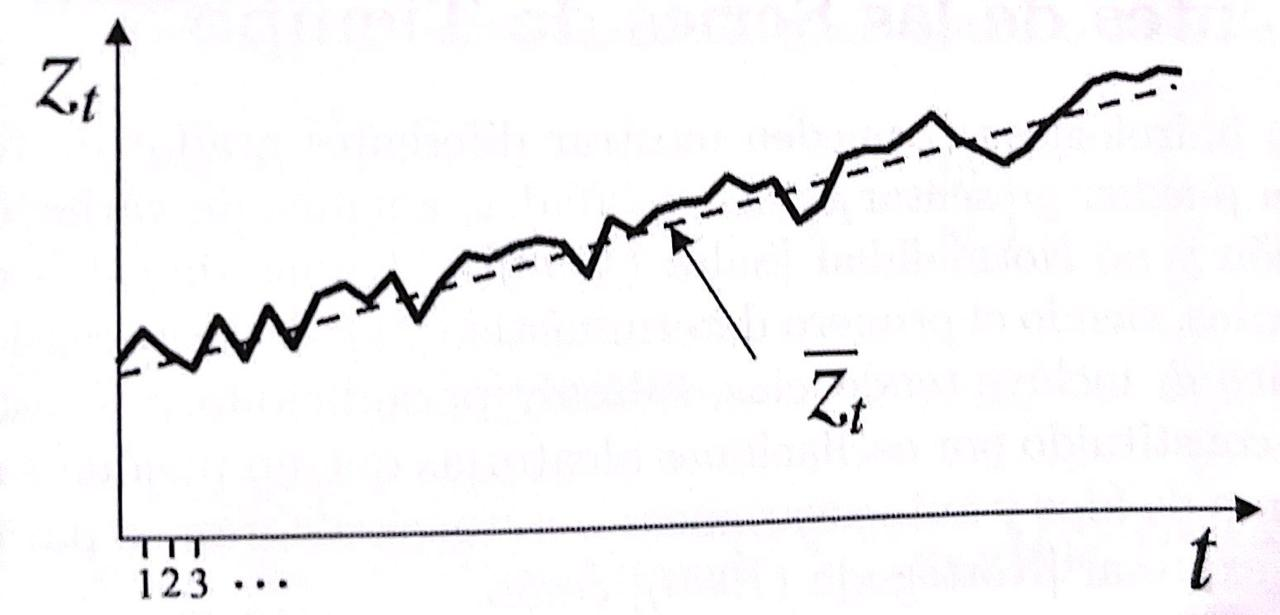
\includegraphics[width=\linewidth]{fiM55.jpeg}  % from Mario Diaz-G
    \end{center}
\end{minipage}
where $\bar{x}(t)$ is the mean of the hydrological time series, $a$, $b$ and $c$ are empirical constants, and $t$ is the time. The figure shows an annual time series with a \emph{positive trend} where the $\bar{x}(t)$ \emph{increase linearly} with time. 
\end{frame}

\begin{frame}{Components of time series}
    \begin{block}{Jumps}
    \end{block}
    \alert{Jumps} are sudden changes in the \emph{mean} and/or in the \emph{variance} often caused by \emph{natural disasters} such as earthquakes, landslides, volcano eruptions and fires. Such changes can be caused by \emph{anthropic events} such as the construction of hydraulic structures (e.g. dams and diversions). \emph{Jumps} can be mathematically represented by
    \[
        \bar{x}(t) = \left\{ \begin{array}{l}  \bar{x}_1 \text{, if } t\leq t^*  \\ \bar{x}_2 \text{, if } t>t^* \end{array} \right. \quad \quad s(t) = \left\{ \begin{array}{l}  s_1 \text{, if } t\leq t^*  \\ s_2 \text{, if } t>t^* \end{array} \right. 
    \]
    where $\bar{x}(t)$ and $s_t$ are the \emph{mean} and the \emph{standard deviation} before and after of $t^*$ (see the figure). 
    \vspace{-4pt}
    \begin{center}
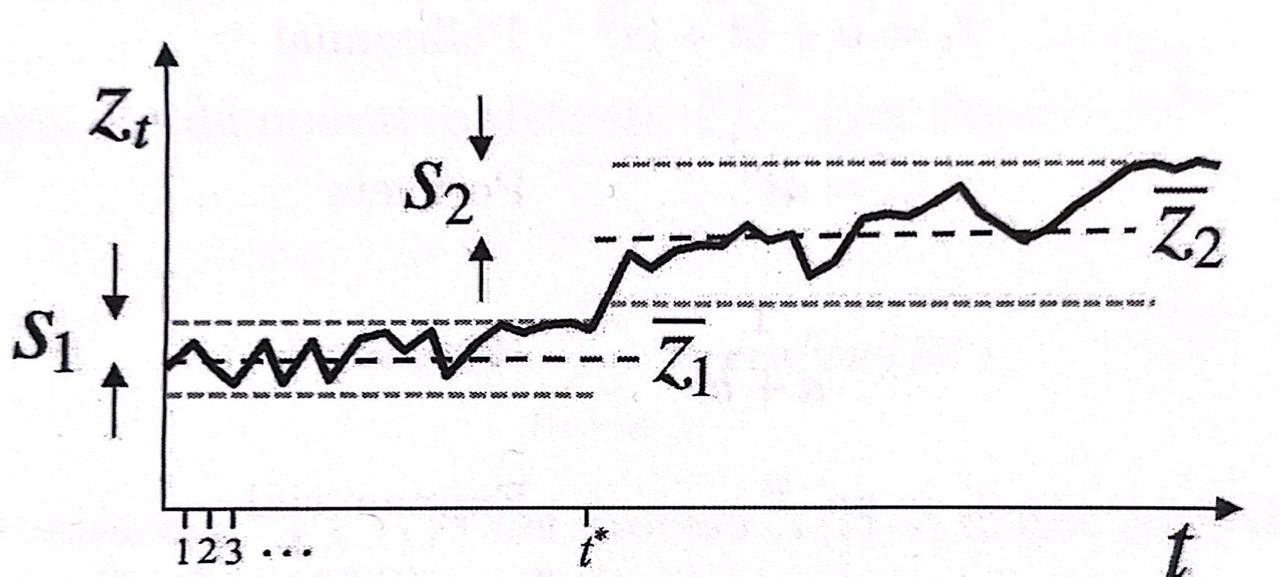
\includegraphics[width=0.9\linewidth]{fiM56.jpeg}  % from Mario Diaz-G
    \end{center}
    \vspace{-4pt}
    Note that the figure shows changes in the \emph{mean} and in the \emph{variance} due to a jump occurred at time $t^*$ caused by a natural and/or anthropic event.  
\end{frame}

\begin{frame}{Components of time series}
    \begin{block}{Trend and jump removal in annual series}
    \end{block}
    Apart from assuming that the data set is \emph{stationary} and \emph{ergodic}, a time series must be free of \emph{trends}, \emph{jumps}, \emph{periodicity}, etc prior being used. So that, the time series must be \emph{transformed} in case such features are present in order to be used in modelling and forecasting. In consequence, \emph{trends}, and \emph{jumps} in \emph{mean} and \emph{variance} in time series with no seasonality can be removed as
    \[
        x'(t) = \frac{x(t)- \bar{x}(t)}{s(t)}
    \]
    where $x(t)$ is the original series, $\bar{x}(t)$ is the \emph{trend} of the \emph{mean} represented by a function, or the \emph{jump} in the \emph{mean}, $s(t)$ is the \emph{trend} in the \emph{variance} represented by function (similar to the functions for the mean), or the \emph{jump} in the \emph{variance}, and $x'(t)$ is the resulting time series after removing \emph{trends} and \emph{jumps} in the \emph{mean} and in the \emph{variance}. 
\end{frame}

\begin{frame}{Components of time series}
    \begin{block}{Periodicity}
    \end{block}
    \vspace{-2pt}
    Sub-annual hydrological time series such as monthly  time series can exhibit \emph{periodic} or \emph{cyclic} patterns as a consequence to the Earth translation around the Sun. This also drive the annual cycle of many hydrological processes. \emph{Periodic} patterns can arise in sub-daily (e.g. hourly) time series due to the daily cycle due to the Earth rotation. Such \emph{periodic} changes are presented in the \emph{mean}, \emph{variance}, \emph{covariance} and \emph{bias} 

    The figure below shows a three-month time series where one year is divided in 4 periods (e.g. seasons) of three months. Note that each period has its \emph{mean} $\bar{x}_j$ and \emph{standard deviation} $s_j$. The time series exhibit a \emph{periodic} behaviour which is not presented in annual time series. 

    \vspace{-5pt}
    \begin{center}
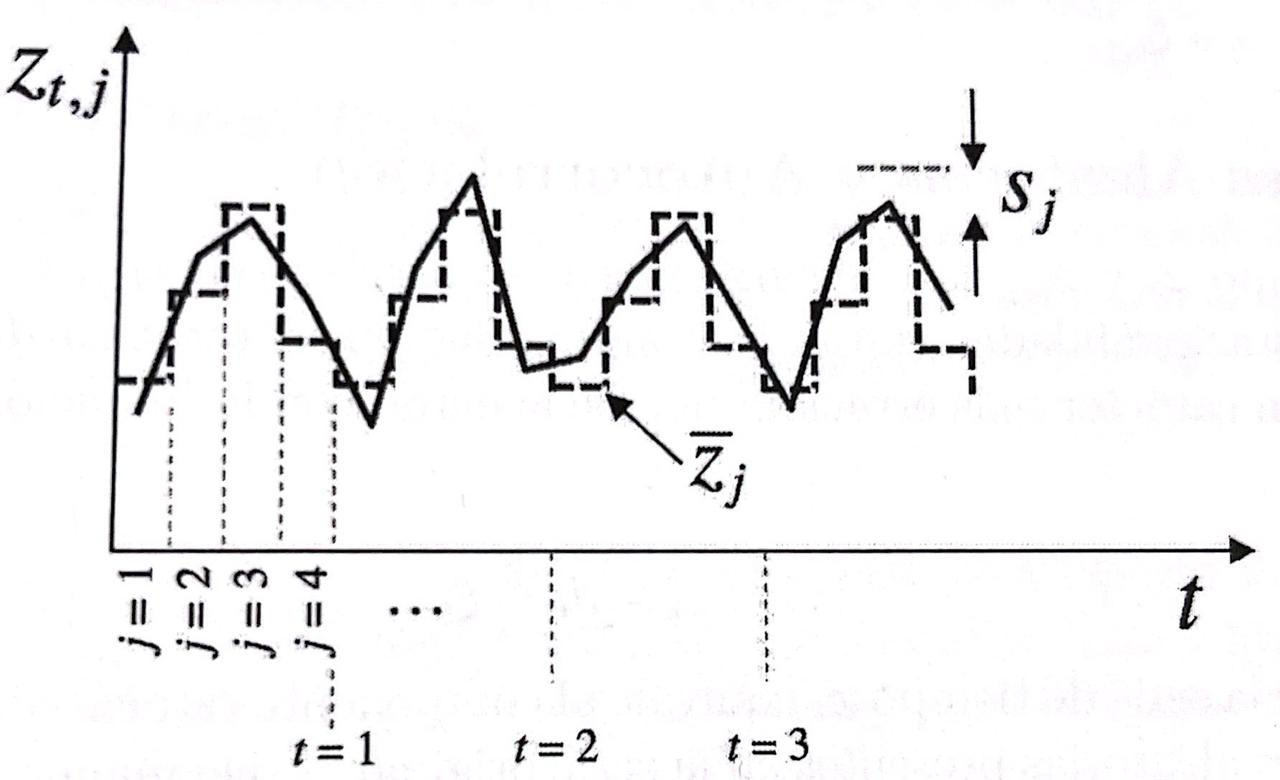
\includegraphics[width=0.8\linewidth]{fiM57.jpeg}  % from Mario Diaz-G
    \end{center}
\end{frame}

\begin{frame}{Components of time series}
    \begin{block}{Periodicity}
    \end{block}
    The \emph{periodicity} in a time series can be represented by a set of sinusoidal functions. So, if the time series $x_j (t)$ does not have \emph{trends} and \emph{jumps}, just the periodicity, this can be represented as
    \[
        x_j (t) = \bar{x} + \sum_{i=1}^L \lambda_i \sin\left\{\frac{2\pi\left[(t-1)n + j\right]}{T} i + \phi_i \right\} + \xi_j (t)
    \]
    where $\bar{x}$ is the \emph{mean}, $n$ is the number of periods is one year ($j=1,\cdots,n$), $L$ is the number of \emph{harmonics} (or \emph{sinusoidal functions}) in one year, $\lambda_i$ and $\phi_i$ are the \emph{amplitude} and the \emph{phase} of each harmonic $i$, and $\xi_j (t)$ is the random component. Regarding that $x_j (t)$  is discrete in time, if $N$ is the length of the time series, the maximun number of harmonics is $L = N/2$ is $N$ is even and $L = N/2-0.5$ if $N$ is odd. In practice, the periodicity is usually represented between one and two harmonics in monthly time series and  between four and six harmonics in daily time series.
\end{frame}

\begin{frame}{Components of time series}
    \begin{block}{Periodicity}
    \end{block}
    \alert{Trends, jumps and periodicity removal in means and variances}\\

    Similarly to annual series with \emph{trends} and \emph{jumps}, these can be removed in series with periodicity. Since there are different \emph{means} and \emph{variances} for each period $j$ of the year, such features can be removed as follow
    \[
        x'_j (t) = \frac{x_j(t)-\bar{x}_j (t)}{s_j (t)}
    \]
    where $x_j (t)$ is the original series, $\bar{x}_j (t)$ is the \emph{mean} during the period $j$ in $t$, $s_j (t)$ is the \emph{standard deviation} in the period $j$ in the time $t$, and $x'_j (t)$ is the resulting standardized time series. If the time series does not have neither \emph{trends} nor \emph{jumps} in the \emph{means} and \emph{variances}, $\bar{x}_j (t) =\bar{x}_j$ and $s_j (t) = s_j$, which means that each period $j$ has constant \emph{mean} and \emph{variance} but different for each $j$. 
    For a \emph{periodic} time series with no \emph{trends} and/or \emph{jumps} in the \emph{means} and \emph{variances} in the $j$ periods, a another way to remove the \emph{periodicity}  from the original series time series is substract the deterministic component as 
    \[
        x'_j (t) = x_j (t) - \bar{x} - \sum_{i=1}^L \lambda_i \sin\left\{\frac{2\pi\left[(t-1)n + j\right]}{T} i + \phi_i \right\} 
    \]
    Note that in this equations $x'_j (t) \equiv \xi_j (t)$.

\end{frame}

\begin{frame}{Components of time series}
    \begin{block}{Random fluctuations and autocorrelation}
    \end{block}
    If the series $x(t)$ and $x_j (t)$ are transformed into $x' (t)$ and $x'_j (t)$, respectively, the last ones are series without \emph{trends}, \emph{jumps} and \emph{periodicity} (these three components constitute the deterministic component $d(t)$ of the time series) and are also \emph{stationary}. Accordingly, the time series $x'(t)$ is
    \[
        x'(t) = x(t)-d (t) = \xi (t)
    \]
    which indicate that $x' (t)$ is equivalent to the random variations presented in the original time series $x (t)$. Similarly the time series $x'_j (t)$ is
    \[
        x'_j (t) = x_j (t)-d_j (t) = \xi_j (t)
    \]

    Note that $x' (t)$ and $x'_j (t)$ can have a structure of \emph{temporal dependency} known as \alert{autocorrelation} that establishes that the magnitude of the hydrological variable depends on its previous values, this means that the process has a form of \alert{'memory'}, frequently called \alert{persistence}. The \emph{persistence} indicates that low (high) values tend to be followed by low (high) values. In any \emph{stochastic process} this temporal dependency is demonstrated through the \emph{autocovariance function} or the \emph{autocorrelation function}. For a \emph{stationary} process, these two function depends only from the temporal lag $\tau$. 
\end{frame}

\begin{frame}{Components of time series}
    \begin{block}{Random fluctuations and autocorrelation}
    \end{block}
    In the case of $x'(t)$, its linear temporal dependency structure is encapsulated in the \alert{correlogram} (\emph{autocorrelation function}), which is a plot of the \emph{correlation} $\rho_k$ vs the lag $k$. For the time series $x'_j (t)$, $k$ represent the number of periods $j$ in the years. For instance, for monthly time series it is possible to obtain 12 \emph{correlograms}, one $\rho_{k,j}$ vs $k$ relationship by month $j$. The coefficients $\rho_{k,j}$ correspond to the correlation of all values in $j$ with  all the values in the lagged month $k$. Note that when a \emph{correlogram} decrease rapidly to zero after few $k$, this show a short \emph{persistence} or \emph{memory}. The opposite occurs when the \emph{correlogram} decrease slowly.\\ 

    \alert{Autocorrelation removal}\\ 

    The removal of the linear temporal dependency structure requires an mathematical model that represent the \emph{correlogram}. The most simple model is a \emph{autoregressive stochastic model} of lag 1. According to this model, the \emph{annual transformed time series} can be expressed as
    \[
        x'(t) = \rho_1 x'(t-1) + \varepsilon (t)
    \]
    where $\rho_1$ is the \emph{correlation coefficient} for lag $k=1$ and $\varepsilon (t)$ is the \alert{residual time series} with no \emph{autocorrelation} (pure stochastic values). $\varepsilon (t)$ is represented by a \emph{pdf} $f_{\varepsilon} (\epsilon)$ which is usually the \emph{Normal distribution}. 
\end{frame}

\begin{frame}{Components of time series}
    \vspace{-5pt}
    \begin{block}{Random fluctuations and autocorrelation}
    \end{block}
    \vspace{-5pt}
    The figures below show some \emph{correlograms} for the streamflow data at the El Banco station in the Magdalena River. 

\begin{minipage}[]{0.48\textwidth}
    \emph{Correlogram} of annual streamflows. $\rho$ decay rapidily after $k>0$, e.g $\rho_1 =0.14$.
\end{minipage}
\hfill
\begin{minipage}[]{0.48\textwidth}
    \begin{center}
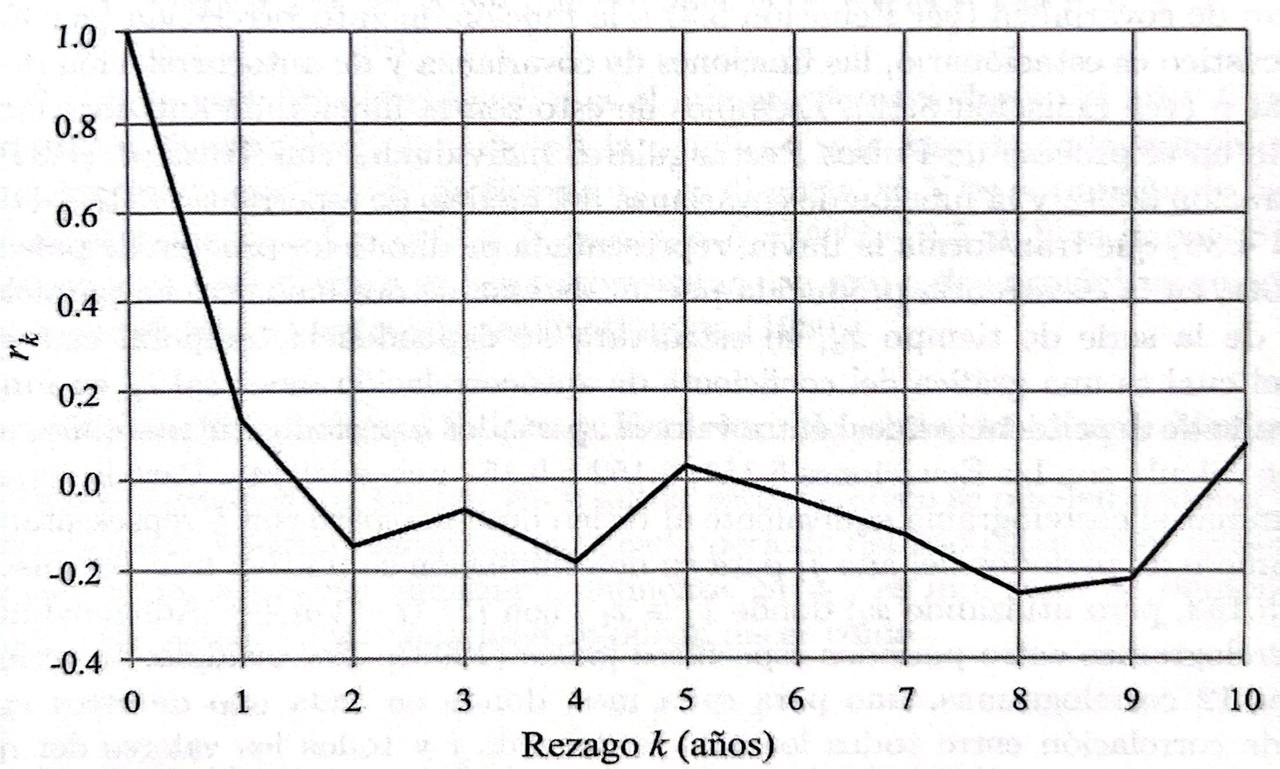
\includegraphics[width=0.8\linewidth]{fiM58.jpeg}  % from Mario-Diaz
    \end{center}
\end{minipage}
 \begin{minipage}[]{0.48\textwidth}
    \emph{Correlogram} of monthly streamflows. There is a large dependency and show periodicity, e.g. $\rho_1 =0.683$ explaining by the bimodal regime of the basin. 
\end{minipage}
\hfill
\begin{minipage}[]{0.48\textwidth}
    \begin{center}
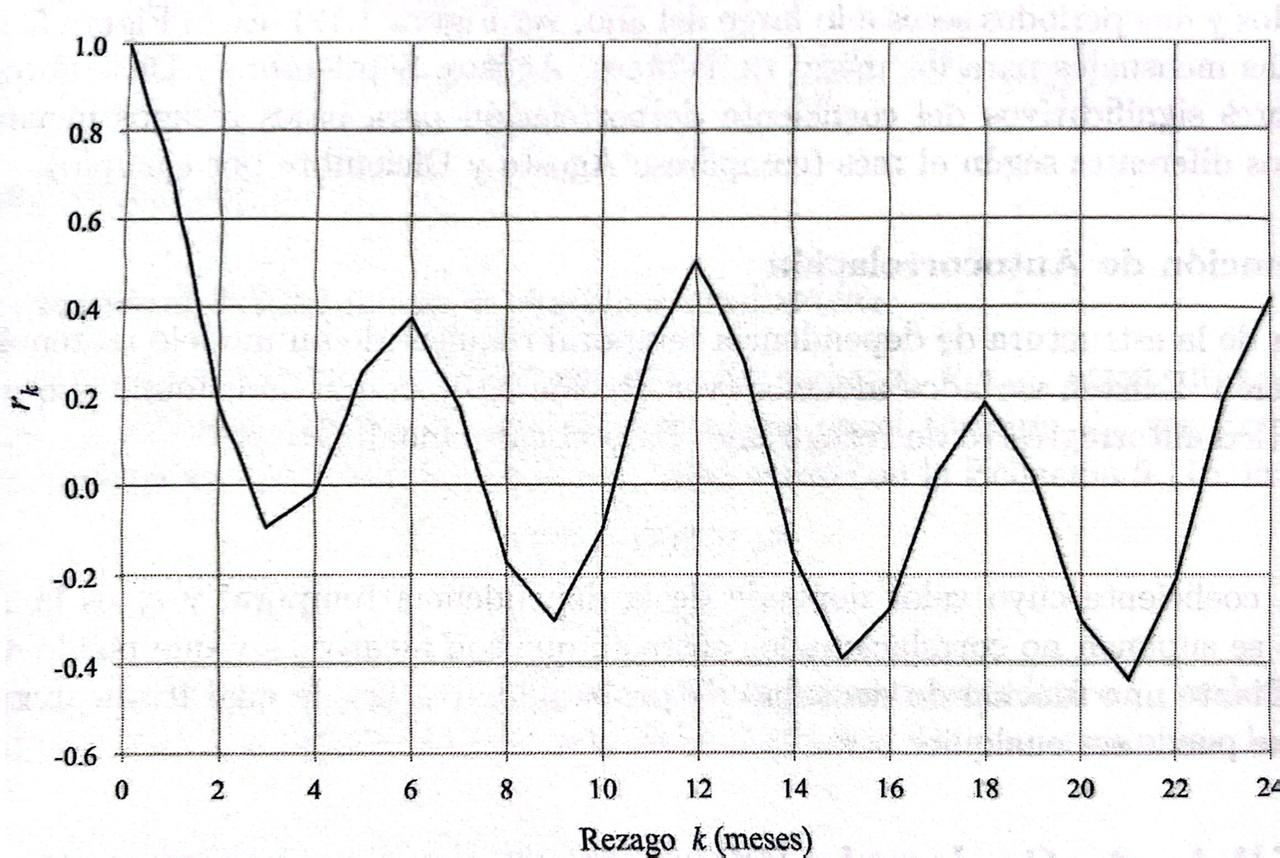
\includegraphics[width=0.8\linewidth]{fiM59.jpeg}  % from Mario-Diaz
    \end{center}
\end{minipage}
 \begin{minipage}[]{0.48\textwidth}
     Monthly \emph{correlograms} of streamflows. Strong dependency in the firsts $k$ and the behaviour of the  \emph{correlogram} is different for each month. 
\end{minipage}
\hfill
\begin{minipage}[]{0.48\textwidth}
    \begin{center}
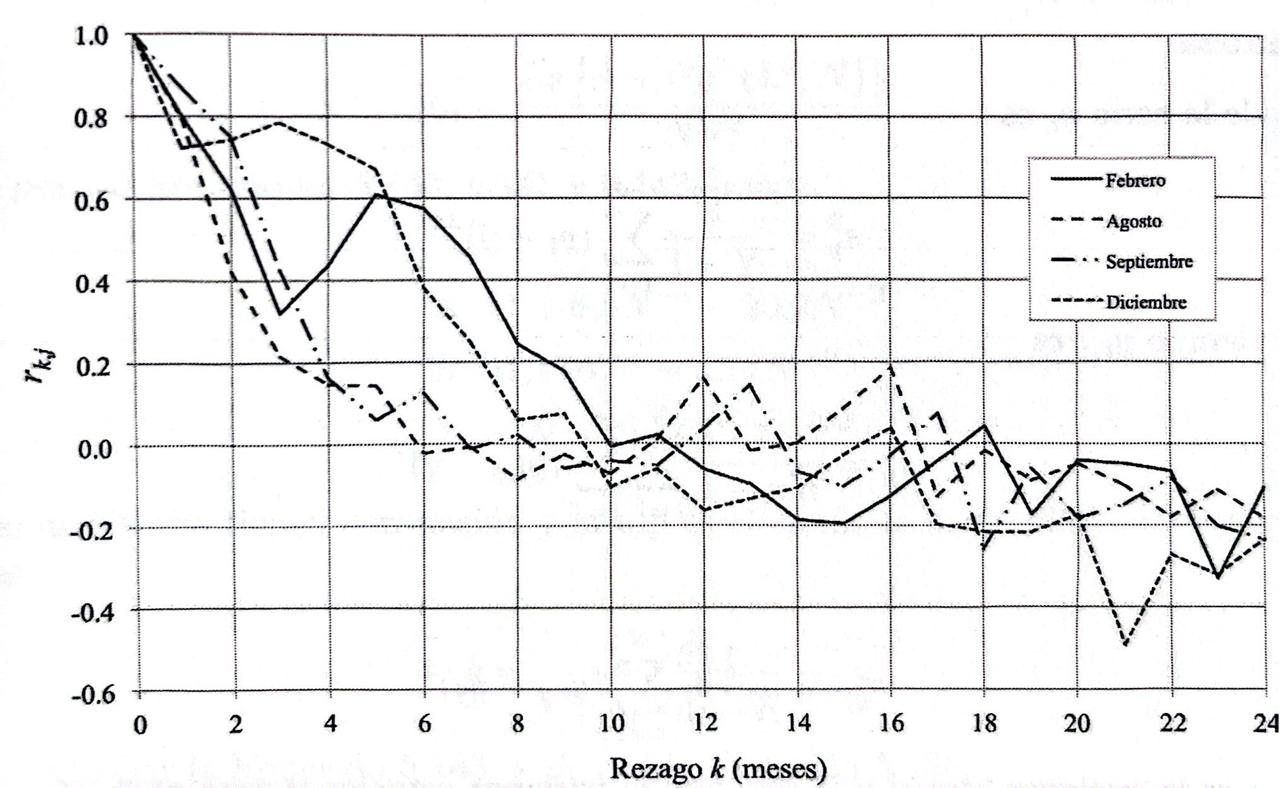
\includegraphics[width=0.8\linewidth]{fiM510.jpeg}  % from Mario-Diaz
    \end{center}
\end{minipage}
\end{frame}

%-------
% From Kotte (Stochastic water r.)
\section{Empirical modal decomposition}
\begin{frame}{Empirical modal decomposition}
\begin{minipage}[]{0.48\textwidth}
    \begin{itemize} 
        \item Procedure developed by Huang et al 1998 that allow to decompose a time series in a finite number of \emph{Intrinsic Modal Functions} with zero Mean.
        \item This functions are associated with different oscillatory modes embedded in the original series. 
        \item The procedure is applied to \emph{no linear} and \emph{no stationaty} time series.
        \item During the decomposition is suppose that the series in any time $t$ is composed for various oscillatory modes of different frequencies overlapping each other. 
        \item The figure (panel a) shows the monthly streamflow in the Las Huertas station at the Bogota River. In the panel (d) is possible to know see the bimodal annual regime and in the panel (h) is possible to detect the macro climatic ENSO signal. 
    \end{itemize} 
\end{minipage}
\hfill
\begin{minipage}[]{0.48\textwidth}
    \begin{center}
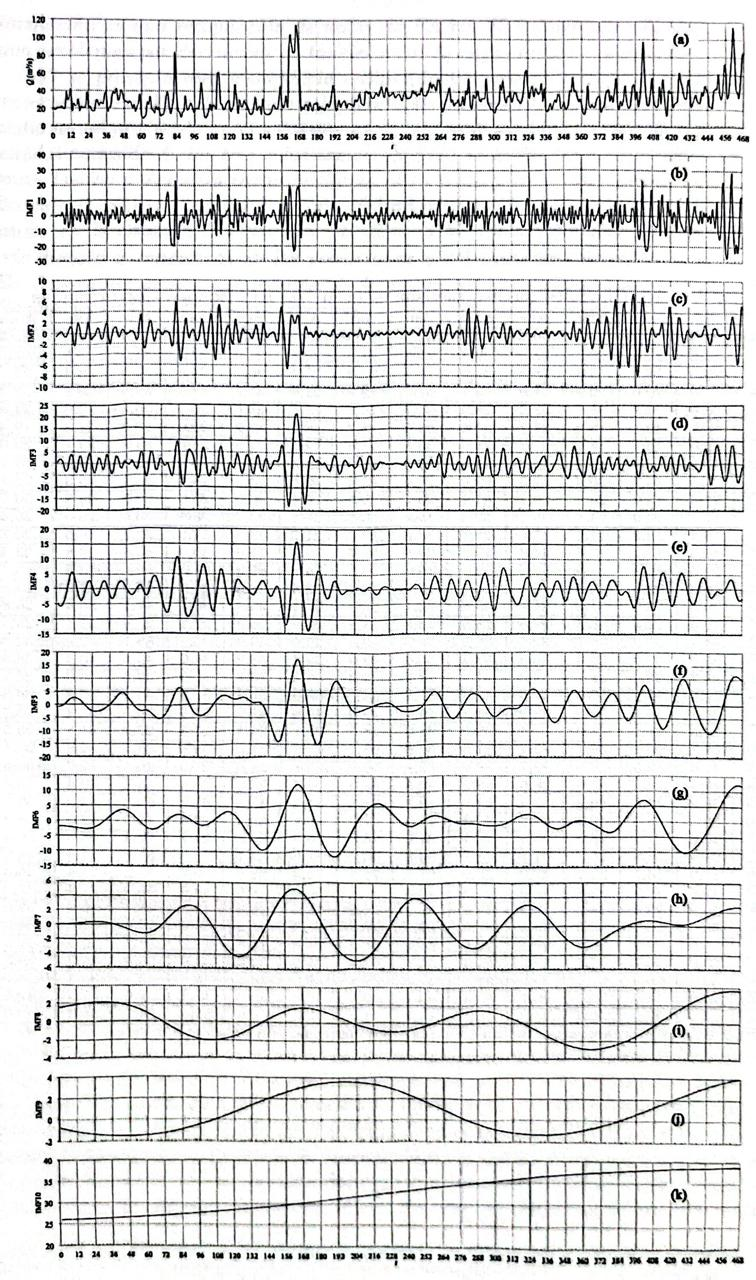
\includegraphics[width=\linewidth]{fiM527.jpeg}  % from Mario Diaz-G
    \end{center}
\end{minipage}

\end{frame}

%-------
% From Kotte (Stochastic water r.)
\section{Test for randomness and trend}
\begin{frame}{Test for randomness and trend}
In certain cases de presence of \emph{trend} or \emph{seasonality} is quite obvious, but often there is doubt whether the suspected effects are significant or not. 
\begin{block}{Turning point test}
\end{block}
    \begin{itemize}
        \item This is a test for \emph{randomness}. 
        \item So in an observed sequence $x(t)$, $t=1,2,\cdots,N$, a \alert{turning point} $p$ occur at time $t=i$ if $x(i)$ is either $x(i+1)$ and $x(i-1)$ or less than the two adjacent values. 
        \item If we consider  three unequal observations, the six possible orders of magnitude of these are: 1. $x(i-1)>x(i) > x(i+1)$, 2. $x(i-1)>x(i+1)>x(i)$, 3. $x(i) > x(i-1) > x(i+1)$, 4. $x(i) > x(i+1) > x(i-1)$, 5. $x(i+1) > x(i-1) > x(i)$ and 6. $x(i+1) > x(i) > x(i-1)$. 
        \item In a random series, the six cases are equally probable and \emph{turning points} occur in all except cases 1 and 6, which means that the chance of  getting a \emph{turning point} is \emph{2/3}. 
        \item Note also that, a \emph{turning point} cannot occur when either $t=1$ or $t=N$. So, the expected number of points in a random series is $E(p) = \frac{2(N-2)}{3}$ and the $Var(p) = \frac{16N-29}{90}$. 
        \item $p$ can be treated as an \emph{standard measure} $z=\frac{p-E[p]}{(Var[p])^{1/2}}$, treated as an \emph{standard normal deviate}. Note that $p$ in $z$ is the number of $p$s from the observations. 
        \item Because too few or too many turning points indicate \emph{non-randomness} (\emph{null hypothesis}), a \emph{two-tailed test of significance is used}.
    \end{itemize}
\end{frame}

\begin{frame}{Test for randomness and trend}
\begin{block}{Kendall's rank correlation test}
\end{block}
    \begin{itemize}
        \item This test is based on the proportionate number of subsequent observations which exceed a particular value. 
        \item For a sequence $x(1), x(2), \cdots, x(N)$, the standard procedure is to determine the number of times, say, $p$, in all pairs of observations ($\{x(i),x(j)\}$, $j>i$) that $x(j)>x(i)$. 
        \item The ordered $(i,j)$ subsets are $(i=1, j=2,3,\cdots,N)$, $(i=2, j=3,4,\cdots,N)$ $\cdots$ $(i=N-1, j=N)$. 
        \item Note that the \emph{maximum possible number} of such pairs occurs for a continuously increasing sequence. This is \emph{rising trend} where succeeding values are throughout greater than preceding ones and $p$ is given by $(N-1)+(N-2)+ \cdots + 1$ which is the sum of an arithmetic progression given by $(N-1)N/2$.
        \item If the observations are totally reversed, $p=0$ and it follows that for a \emph{trend-free series} $E[p] = N(N-1)/4$. 
        \item Note therefore that, if $p$ is close to $(N-1)N/2$ or 0, it indicates the presence  of a \emph{raising} or \emph{falling} trend, respectively. 
        \item The test is based on the $\tau = \frac{4p}{N(N-1)} -1 $ statistics for which $E[\tau] =0$ and $Var[\tau] = \frac{2(2N+5)}{9N(N-1)}$, and that $\frac{\tau}{(Var[\tau])^{1/2}}$ converges rapidly to a \emph{standard normal distribution} as $N$ increases. Note that this relationship is thus the \emph{standard test statistics}. 
        \item The \emph{null hypothesis} is of \emph{no trend} in the series, and a \emph{two-tailed test of significance is used}. 
    \end{itemize}
\end{frame}
 
\begin{frame}{Test for randomness and trend}
    \begin{block}{Regression test for linear trend}
\end{block}
    \begin{itemize}
        \item This test is useful when it is thought that the \emph{trend} is approximately \emph{linear}. Standard methods of \emph{linear regression} are used for this purpose. 
        \item According to the expression for the \emph{linear model}  $X(t) = x_0 + \alpha t + \varepsilon (t)$, the hypothesis to be tested is $\alpha \neq 0$
        \item The first step is to estimate $\alpha$ and its variance denoted as $\hat{\alpha}$ and $s_{\hat{\alpha}}^2$, respectively. 
        \item The statistics $t = \frac{\hat{\alpha}}{s_{\hat{\alpha}}^2}$ is then tested by using \emph{Student's t test}. It is assumed here (as in other types of \emph{regression analysis})  that the \emph{residuals} $\varepsilon (t)$ are \emph{stationary}, sequentially \emph{independent} and \emph{normally distributed}.  
        \item The \emph{null hypothesis} is of $\alpha=0$ (\emph{no trend}). So the statistics $t$ is calculated and compared against the values from the \emph{Student's t test}.  
    \end{itemize}
    Other considerations:
    \begin{itemize}
        \item Note that \emph{linearity} in \emph{trend} is mainly a theoretical concept used to describe a general pattern, where \emph{trends} in natural time series are \emph{non-linear}. 
        \item Also, \emph{hydrologic time series} are not subject to \emph{long-term movements}, generally speaking, over observed time spans. So, most of the exceptional cases appear to be caused by \emph{local changes} in \emph{physical conditions} (e.g catchment deforestation).
    \end{itemize}
\end{frame}
 

%-------
% From Bierkens
\section{Moments and expectation}

\begin{frame}{Moments and expectation}
    A single time series is considered a \emph{stochastic process} that can be characterized  by its (central) \emph{statistical moments}. In particular,  the first and second order moments are relevant: the \emph{mean} value, the \emph{variance} and the \emph{autocorrelation} function. For an statistical \emph{stationary process} the \emph{mean} and the \emph{variance} are:
    \[
        \mu_X = E[X(t)] \quad \quad \sigma_X^2 = Var[X(t)] = E\left[(X(t)-\mu_X )(X(t) - \mu_X)\right]
    \]
    The \emph{autocovariance} is a measure of the relationship of the process at two points in time. For two points in time $k$ time steps apart, the \emph{autocovariance} is defined by
\[
    COV[X(t), X(t+k)] = E\left[(X(t)-\mu_X )(X(t+k) - \mu_X)\right] \quad k=-\infty,\cdots,-1,0,1,\cdots,\infty
\]
where $k$ is often called \emph{time lag}. Note that when $k=0$  $COV[X(t), X(t+k)]=\sigma_X^2$ and $COV[X(t), X(t+k)]=COV[X(t+k), X(t)]=COV[X(t), X(t-k)]$

In \emph{time series analysis} we often  use the \emph{autocorrelation function (acf)}defined by
\begin{align*}
    \rho_{XX,k} &=\frac{COV[X(t), X(t+k)]}{ COV[X(t), X(t)]} \\
                &= \frac{E\left[(X(t)-\mu_X )(X(t+k) - \mu_X)\right]}{\sigma_X^2}\quad k=-\infty,\cdots,-1,0,1,\cdots,\infty
\end{align*}
Note that \emph{acf} is always between 1 and -1, so a value of 1 or -1 \emph{means} a \emph{perfect correlation}, while a value 0 indicates the \emph{absence of correlation}. From the definition it follows that the \emph{acf} is maximum for $k=0$ ($\rho_{XX,0} =1$). Just like for the \emph{autocovariance} it follows from the definition that $\rho_{XX,k} = \rho_{XX,-k}$ $k=-\infty,\cdots,-1,0,1,\cdots,\infty$.
\end{frame}

\begin{frame}{Moments and expectation}
    Different characteristics of zero mean time series due to high and low values for the \emph{variance} and the \emph{acf}.  Note that the \emph{dynamic behavior} of a time series is characterized by these two features.
    \begin{center}
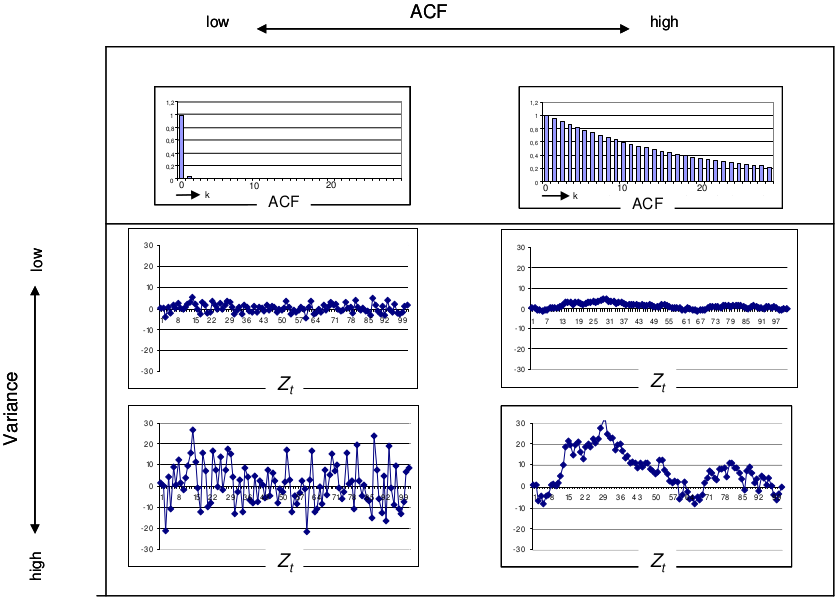
\includegraphics[width=\linewidth]{fiBi62.png}  % from Bierke
    \end{center}
\end{frame}


\begin{frame}{Moments and expectation}
    Analogous to the \emph{autocovariance} and the \emph{acf}, that expresses the relation of a time series with itself, the relation between two different time series is expressed by the \emph{cross covariance} and the \emph{crosscorrelation function (ccf)}. The \emph{cross covariance} and \emph{ccf} for the time series $X(t)$ and $Z(t)$ is defined as:
    \[
        COV[X(t), Z(t+k)] = E\left[(X(t)-\mu_X) (Z(t)-\mu_Z)\right]
    \]

    \[
    \rho_{XZ,k} =\frac{E\left[(X(t)-\mu_X) (Z(t)-\mu_Z)\right]}{\sigma_X \sigma_Z}
\]
Analogous to the \emph{acf}, the value of the \emph{ccf} is always between 1 and
-1. However the \emph{ccf} is \emph{not symmetrical} around $k=0$: $\rho_{XZ,k}\neq\rho_{XZ,-k}$. However, from the definition of \emph{ccf} $\rho_{XZ,k}\neq\rho_{ZX,-k}$. 

%In the real world we don't know the process $X(t)$ exactly and we have to estimate all information from \emph{observations}. In absence of observation errors, the observation $x(t)$ equals the value of the process $X(t)$ . Suppose we have observations of the process from \emph{time step 0} until \emph{time step $t$}.

\end{frame}

%-------
% From Bierkens
\section{Dealing with real data}
\begin{frame}{Dealing with real data}
    Here we list some typical question that the anlyst must ask itself for \emph{cleaning} the time series, and to deal with \emph{trend} and \emph{seasonality}.
    \begin{itemize}
        \item Do you \emph{understand} the context? Have the \emph{'right'} variables been \emph{measured}?
        \item Have all the time series been \emph{plotted}?
        \item Are there any \emph{missing values}? If so, what should be done about them? 
        \item Are there any \emph{outliers}? If so, what should be done about them?
        \item Are there any obvious \emph{discontinuities} in the data? If so, what does this mean?
        \item Does it make sense to \emph{transform} any of the variables?
        \item Is \emph{trend} present? If so, what should be done about it?
        \item Is \emph{seasonality} present? If so, what should be done about it?
           
        \end{itemize}
\end{frame}

\end{document}
